\chapter{Stand der Technik}

In diesem Kapitel wird auf den Stand der Technik eingegangen. Im weitesten zitiere ich hier die wissenschaftlichen Paper, auf denen meine Arbeit beruht. Ob man das Kapitel noch weiter einteilen muss, wird sich später zeigen, erstmal lasse ich es ohne Unterkapitel. \\
Mobile Roboter finden immer mehr Einzug in Umgebungen, welche von Menschen bewohnt sind. Diese Menschen üben Aktivitäten aus, welche in der Folge zu Veränderungen eben dieser Umgebung führen. Man kann davon ausgehen, dass viele dieser Aktivitäten täglichen Routinen mit typischen Mustern folgen, welche von mobilen Robotern erkannt werden und zur robusteren Darstellung ihrer Umgebung genutzt werden können. Mapping in statischen Umgebungen stellt ein weit erforschtes Gebiet dar \cite{Eichler.2006}. Für das Mapping in dynamischen Umgebungen gibt es verschiedene Ansätze. Während ein Ansatz darauf abzielt, sich bewegende Objekte aus der Umgebungsdarstellung herauszufiltern \cite{Hahnel.30Sept.5Oct.2002}, werden in anderen diese Objekte getrackt und als bewegte Landmarken klassifiziert \cite{Montesano.2008}. Diese separations-basierten Ansätze können jedoch nicht auf Langzeitveränderungen der Umgebungsstruktur eingehen. \\
Im Gegensatz hierzu stehen adaptive Ansätze, welche davon ausgehen, dass die Karte niemals komplett ist und diese durch kontinuierliches Mapping aktualisieren. So können der Karte durch neue Observierungen des mobilen Roboters neue Features hinzugefügt werden 
\cite{Milford.2010}. In \cite{Krajnik.2014} wird nun erstmalig versucht, die räumlich-zeitliche Dynamik der Umgebung durch ihr Frequenzspektrum darzustellen. Die Zustände von lokalen Umgebungsmodellen, wie zum Beispiel einer Tür, welche entweder offen oder geschlossen sein kann, sollen hier durch Wahrscheinlichkeitsfunktionen repräsentiert werden, welche aus der Superposition periodischer Funktionen entstehen. In \cite{Krajnik.2014} wird als Motivation dazu angeführt, dass die meisten Mapping Ansätze wichtige Komponenten der Umwelt, wie z.B. eine Tür, durch lediglich zwei eindeutige Zustände dargestellt werden. Eine Tür ist also entweder geöffnet oder geschlossen. % Hier noch eine entsprechende Quelle einfügen.\\
Diese Zustände können jedoch auch durch ihre Wahrscheinlichkeit $p_j$ ausgedrückt werden. Bayes-Filter gehen hierzu von einen statischen Welt aus, d.h. die Wahrscheinlichkeiten der Zustände $p_j$ werden als konstant angesehen. Durch neue Beobachtungen können diese konstanten Annahmen verändert werden, alte Beobachtungen werden so jedoch über die Zeit "vergessen" \cite{Krajnik.2014}. Nimmt man jetzt jedoch an, dass diese Zustandswahrscheinlichkeiten Funktionen der Zeit sind, also $p_j (t)}$ gilt, und diesen zeitlichen Veränderungen der Wahrscheinlichkeiten eine finite Nummer periodischer Prozesse zu Grunde liegt, könnte man den Einfluss und die Periodizität eben dieser Prozesse identifizieren und die Zustandswahrscheinlichkeit $p_j (t)$ aus dieser Beschreibung ermitteln. In \cite{Krajnik.2014} wird nun die in Abschnitt \ref{sec:Fourierreihen und Fouriertransformation} erläuterte Fouriertransformation benutzt, um diese periodischen Prozesse zu identifizieren. Als Beispiel wird ein Belegungsnetz herangeführt. Jede der Zellen des Belegungsnetzes kann zwei Zustände $s_j = \{frei, belegt\}$ annehmen. Diese Zustände sind jedoch nicht konstant, sondern eine Funktion der Zeit, also $s_j (t)$. Die Unsicherheit des Zustandes wird nun durch sein Wahrscheinlichkeit $p_j (t)$ ausgedrückt. Da die Zellen unabhängig voneinander sind, kann die Fouriertransformation separat auf jede Zelle des Belegungsnetzes angewendet werden. \\ Die über die Zeit aufgetragenen Zustände einer Zelle $s(t)$ werden mittels der Fouriertransformation $P = FT(s(t))$ transformiert. Es werden l Koeffizienten $P_i$ des Spektrums $P$ ausgewählt und zusammen mit ihren Frequenzen $\omega_i$ benutzt, um mittels der inversen Fouriertransformation $p(t) = IFT(s(t))$ die Wahrscheinlichkeitsfunktion $p(t)$ des Zellzustandes zu bestimmen. Abschließend wird ein Schwellwert benutzt, um aus $p(t)$ eine Schätzung $s'(t)$ der tatsächlichen Zustandsfunktion $s(t)$ zu bestimmen. Das Set $P$ besteht hierbei aus $l$ Tripeln mit den Einträgen $(abs(P_i), arg(P_i), \omega_i)$, wobei $abs(P_i)$ für die Amplitude, $arg(P_i)$ für den Phasenversatz und $\omega_i$ für die Frequenz des jeweiligen periodischen Prozesses steht, welcher den Zustand $s(t)$ beeinflusst. \\

Der Zustand einer Zelle wird nun über die Gleichung xy approximiert. 
\begin{equation}
	s(t) = (IFT(P) > 0.5) \oplus  (t \notin 0)
	\label{eq:Zellzustand}
\end{equation}
Ist die Wahrscheinlichkeit $p(t)$ einer Zellbelegung größer als 0.5, so wird die Zelle als belegt geschätzt, sofern der Zeitpunkt $t$ nicht zum Set der Ausreißer 0 gehört.
%Ausreißer-Set muss noch eingebunden werden.
Der in Gleichung benutzte Schwellwert von 0.5 kann willkürlich gesetzt werden. So können Vorhersagen über zukünftige Zustände der Zelle mit einem gewissen Konfidenzniveau von $c$ durch die Gleichung:
\begin{equation}
	s'(t,c) = IFT(P) > c
	\label{eq:Zustandsvorhersage}
\end{equation}
getroffen werden. Grafisch verdeutlicht wird die Methodik durch \bild{FreMEn Beispiel}. 

\begin{figure}[!ht]
	\begin{center}
		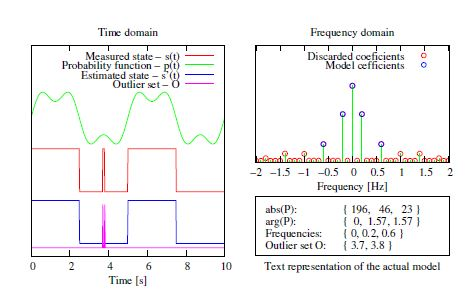
\includegraphics[]{example_of_measured_state_and_prediction}
		\caption{Beispiel eines über die Zeit gemessenen Zellzustandes sowie seines Spektralmodells und Wahrscheinlichkeitsprädiktion Quelle (Krajnik.2014)}
		\label{fig.FreMEn Beispiel}
	\end{center}
\end{figure}
In der linken Grafik rot dargestellt sind die über einen zeitlichen Verlauf aufgenommenen, binären Zustände einer Beispielzelle. Der grüne Graph beschreibt das zugehörige FreMEn-Modell der Ordnung drei. In blau aufgetragen sind die Vorhersagen des Modells ermittelt anhand eines Schwellwertes von 0.5. Der lila Graph stellt die Zeitpunkte dar, zu denen die Modellvorhersage von den tatsächlichen Zellzuständen abweicht \cite{Krajnik.2014}. Die rechte obere Grafik repräsentiert das Frequenzspektrum der Zelle, die für das Modell ausgewählten Frequenzen sind durch blaue Kreise markiert. Das zuvor erwähnte Tripel bestehend aus Amplitude, Phasenversatz und Frequenz der jeweiligen periodischen Prozesse ist in der rechten unteren Grafik dargestellt. Um die Auswirkungen des Modellgrades, also der Anzahl der in das Modell einfliessenden periodischen Prozesse, zu erforschen, wurde die Methodik auf einen Datensatz angewendet, bei welchem ein SCITOS-G5 mobiler Roboter ausgestattet mit RGB-D und Lasersensoren, Personen in einem Bürogebäude über eine Dauer von einer Woche mit einer Rate von \SI{30}{\hertz} detektiert hat. \\
Die Genauigkeit des Modells $q(t_a,t_b)$ wird anhand von Gleichung xy berechnet und beschreibt das Verhältnis von korrekt geschätzten Zellzuständen zu der Gesamtdauer des betrachteten Intervalls.
\begin{equation}
	q(t_a,t_b) = \frac{1}{t_b - t_a} \int_{t_a}^{t_b} |s'(t) - s(t)| \ind{d}t
	\label{eq:Modellgenauigkeit}
\end{equation}
Unterschieden wurde nun in \cite{Krajnik.2014} zwischen dem Rekonstruktionsfehler $q_r$ sowie dem Prädiktionsfehler $q_p$. Der Rekonstruktionsfehler beschreibt, wie genau das Modell Zeitintervalle beschreibt, welche zur Ermittlung der Modellparameter verwendet wurden. Der Prädiktionsfehler hingegen beschreibt die Genauigkeit des Modells in Bezug auf Zeiträume, welche nicht zur Modellermittlung verwendet wurden. Die ermittelte Abhängigkeit des Rekonstruktions-sowie Prädiktionsfehlers von der Modellordnung ist in \bild{Modellgenauigkeit} aufgezeigt. \\
\begin{figure}[!ht]
	\begin{center}
		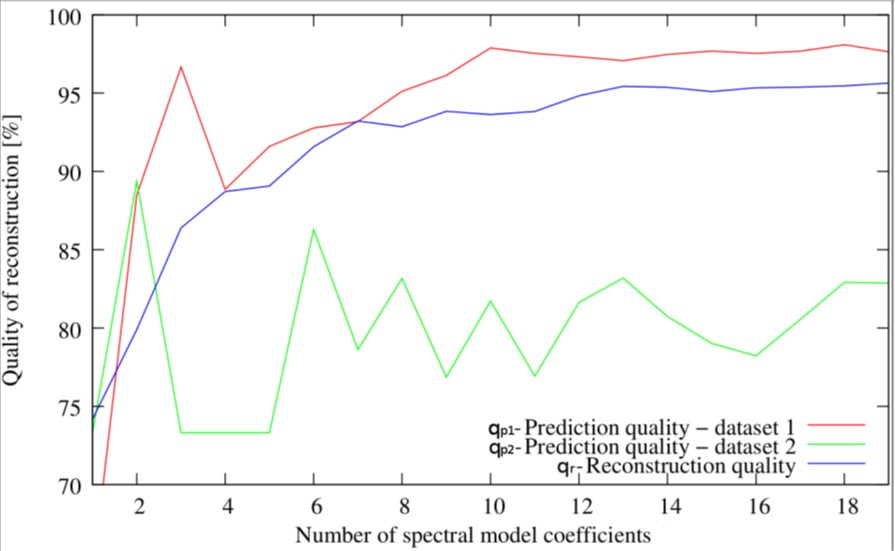
\includegraphics[]{Prediction_Reconstruction_Error}
		\caption{Modellgenauigkeit vs. Modellordnung Quelle (Krajnik.2014)}
		\label{fig.Modellgenauigkeit}
	\end{center}
	
\end{figure}

Die Rekonstruktionsgenauigkeit liegt bei einer Modellordnung von 15, d.h. es wurden 15 periodische Prozesse zum Approximieren des Zustandssignales verwendet, bei 95 \%. Die Rekonstruktionsgenauigkeit $q_r$ steigt dabei monoton mit der Modellordnung, die Prädiktionsgenauigkeit $q_p$ hingegen nicht. % Manchmal nenne ich q_p hier Prädiktionsgenauigkeit und manchmal Fehler, das muss ich noch einheitlich machen. 
\\
Die lokalen Maxima von $q_\ind{p1}$ und $q_\ind{p2}$ lassen den Schluss zu, dass für die Vorhersage eine Modellordnung von zwei oder drei optimal ist (siehe \bild{Modellgenauigkeit}). \\
% \cite{Krajnik.2015b} 
Einen Vergleich zwischen der in \cite{Krajnik.2014} beschriebenen "Frequency Map Enhancement" (FreMEn) Methode und der Anwendung von periodischen Gauß-Mixmodellen zur Darstellung der Dynamik von Umweltzuständen zieht \cite{Krajnik.2015b}. FreMEn basiert hier, wie auch schon in \cite{Krajnik.2014} darauf, die zeitliche Funktion $s(t)$ eines Umweltzustandes durch seine Wahrscheinlichkeitsfunktion $p(t)$ zu schätzen. Auch hier wird wieder mittels einer Fouriertransformation das Frequenzspektrum $S(\omega)$ der zeitlichen Funktion $s(t)$ bestimmt, und die l prominentesten Frequenzen mit ihren Amplituden $a_j$, ihrem Phasenversatz $\varphi_j$ sowie ihrer Frequenz $\omega_j$ abgespeichert. Die Ermittlung der Wahrscheinlichkeit eines Umweltzustandes zum Zeitpunkt t ergibt sich nun durch die Superposition der l Frequenzen mittels Gleichung \ref{eq:Superposition}.
\begin{equation}
	p(t) = a_o + \sum_{j=1}^{n} a_j \cos(\omega_j t + \varphi_j)
	\label{eq:Superposition}
\end{equation}
Die erste spektrale Komponente $a_0$ stellt hierbei den Durchschnitt aller binären Werte von $s(t)$ dar. FreMEn besitze aber laut \cite{Krajnik.2015b} zwei wesentliche Nachteile. So erlaube es zum Einen, lediglich einen periodischen Prozess pro Frequenz zu modellieren. Des Weiteren bilde es wiederkehrende, aber kurze Prozesse, schlecht ab. Als Beispiel wird hier die morgendliche Dusche angeführt, welche eine tägliche, aber kurze Routine sei. Da in \cite{Krajnik.2014} herausgearbeitet wurde, dass die optimale Modellordnung für eine möglichst genaue Prognostizierfähigkeit bei lediglich zwei bis drei liegt, könnten solche kurzen Routinen schlicht nicht abgebildet werden. \\ Als zweiter Ansatz werden Gaussian Mixture Models (GMM) genannt. Diese können multidimensionale Funktionen als gewichtete Summe aus mehreren Gauß-Funktionen mittels Gleichung xy approximieren.
\begin{equation}
	f(t) = \frac{1}{\sqrt{2 \pi}} \sum_{j=1}^{m} \frac{\omega_j}{\sigma_j} e^\ind{- \frac{(t- \mu_j)^2}{2 \sigma_j ^2}}
	\label{eq:Gaussian_Mixture_Models}
\end{equation}
Die Parameter der individuellen Komponenten eines GMM, namentlich das Gewicht $\omega_k$, der Durchschnitt $\mu_j$ sowie die Standardabweichung $\sigma_j$ werden typischerweise mittels Trainingsdaten anhand des Iterative Expectation Maximization (EM) oder des Maximum A-Posteriori (MAP) Algorithmus ermittelt. Während GMM's in der Lage sind, Funktionen jeglichen Aussehens zu modellieren, liegt ihre Limitation darin, dass sie definitionsgemäß keine periodischen Funktionen repräsentieren können \cite{Krajnik.2015b}. Um diesem Problem entgegenzuwirken, wird vorab eine Periode von einem Tag vorgegeben. Diese Vorgabe erlaubt es, die gemessene Sequenz der Umweltzustände $s(t)$  in eine Sequenz $p'(t)$ umzuwandeln.
\begin{equation}
	p'(t) = \frac{k}{\tau} \sum_{i=1}^{\frac{k}{\tau}} s(t+i \tau)
	\label{eq:GMM_sequence}
\end{equation}
In Gleichung \ref{eq:GMM_sequence} bezeichnet [$\tau$] die vorab definierte Periodendauer, $k$ beschreibt die Länge der Sequenz $s(t)$. Nach Anwendung des Expectation Maximization Algorithmus kann nun die Wahrscheinlichkeit für einen Umweltzustand mittels Gleichung \ref{eq:Gauss_Probability} berechnet werden. 
\begin{equation}
	p(t) = \frac{1}{\sqrt{2 \pi}} \sum_{j=1}^{m} \frac{w_j}{\tau_j} e ^\ind{- \frac{(mod(t,\tau) - \mu_j)^2}{2 \sigma_j^2}}
	\label{eq:Gauss_Probability}
\end{equation}
Hierbei beschreibt $\tau$ die vorgegebene Periodendauer der Funktion $p(t)$ und $mod$ ist der Modulo-Operator. Dass die Stärken und Schwächen dieser periodischen GMM-basierten (PerGaM) Modelle komplementär zu denen der FreMEn-Methodik sind, wir anhand von \bild{PerGaM_vs_FreMEn} deutlich.
\begin{figure}[!ht]
	\begin{center}
		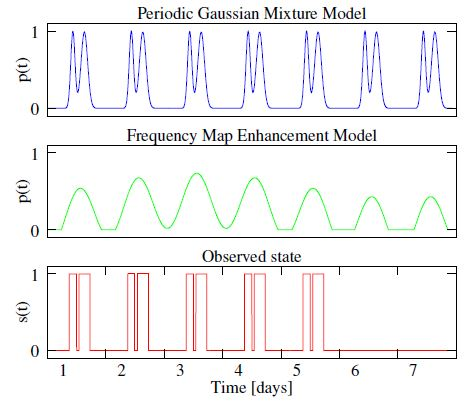
\includegraphics[]{PerGaM_vs_FreMEn}
		\caption{PerGaM und FreMEn Modellvergleich Quelle (Krajnik.2015b)}
		\label{fig.PerGaM_vs_FreMEn}
	\end{center}
\end{figure}
Das PerGaM-Modell kann selbst kurze, mehrfache Events approximieren, jedoch kann es lediglich eine Periodendauer repräsentieren, welche a priori (im Vorhinein) bekannt bzw. festgelegt werden muss. Als Resultat werden kurzzeitige Events, wie z.B. Mittagspausen, gut approximiert, die wöchentliche Dynamik mit dem Fehlen von Personen am Wochenende kann hingegen jedoch nicht modelliert werden. Im Vergleich dazu sieht man das FreMEn-Modell, welches diese Wochendynamik durch ein Abflachen der Signalamplitude an den beiden Wochenendtagen abbildet (siehe \bild{PerGaM_vs_FreMEn}). \\
In Bezug auf die zeitlich-räumliche Kartierung durch mobile Roboter führt \cite{Krajnik.2015} an, dass dieses auch eine räumlich-zeitliche Explorationsstrategie benötigt. Im Vergleich zu klassischen Explorationsstrategien, bei denen, bedingt durch die endliche Größe der zu erforschenden Karte, die Exploration ebenfalls finit ist, sei die Exploration dynamischer Umgebungen niemals abgeschlossen. Vielmehr bekäme die räumlich-zeitliche Exploration Teil der täglichen Routine des Roboters.
Es stellt sich ein wesentlicher Nachteil der in \cite{Krajnik.2014} vorgestellten Methode zur Darstellung von Umweltzuständen in Bezug auf die kontinuerliche Exploration einer Karte durch einen mobilen Roboter. Diese beruht ja auf der traditionellen Fast Fourier Transformation (FFT). Die Fast Fourier Transformation kann jedoch lediglich die komplette Sequenz eines Umweltzustandes $s(t)$ in sein Frequenzspektrum $S(\omega)$ transformieren. Außerdem erfordert der Algorithmus, dass die Zustandsobservierungen mit der immer gleichen Frequenz aufgenommen werden.  Orte mit der immer selben Frequenz zu erkunden, sei jedoch nicht effizient, sodass in \cite{Krajnik.2015} eine neue Methode zur Darstellung von Umweltzuständen durch zeitlich variable Wahrscheinlichkeitsfunktionen vorgestellt wird. Die Methode erlaubt ein inkrementelles und kontinuierliches Aktualisieren des räumlich-zeitlichen Umgebungsmodells durch wenige Observierungen, welche zu unterschiedlichen, nicht gleichmäßig verteilten Zeitpunkten, und an unterschiedlichen Orten aufgenommen werden können. \\
Jeder Umweltzustand wird nun durch die Nummer getätigter Observierungen $n$, seines Durchschnittes $\mu$ sowie zwei Sets $A,B$ komplexer Zahlen $\alpha_k$ und $\beta_k$, welche zu dem Set $\Omega$ periodischer Prozesse $\omega_k$ gehören, welche den Umweltzustand beeinflussen. Anfangs wird der Wert $\mu$ zu 0.5 und alle $\alpha_k$ sowie $\beta_k$ zu 0 gesetzt, was einem vollkommen unbekannten Zustand entspricht. Die inkrementelle Aktualisierung des Modells erfolgt nun anhand von Gleichung \ref{eq:Update_step_FreMEn}.
\begin{align}
	\mu &\leftarrow \frac{1}{n+1}(n \mu + s(t)), \\
	\alpha_k &\leftarrow \frac{1}{n+1} (n \alpha_k + s(t) e^\ind{-jt\omega_k})  &\forall \omega_k \in \Omega, \\
	\beta_k &\leftarrow \frac{1}{n+1} (n \beta_k + \mu e^{ind{-jt\omega_k}})  &\forall \omega_k \in \Omega, \\
	n &\leftarrow n + 1
	\label{eq:Update_step_FreMEn}
\end{align}


